%************************************************
\chapter{Progettazione}\label{ch:progettazione}
%************************************************
Il seguente capitolo descrive le scelte progettuali che sono state effettuate, ovvero viene presentata l'architettura generale di \emph{Sencha Touch} e dei prototipi \emph{MyNotes} e \emph{SensorDevice} attraverso diagrammi delle classi.

\section{Sencha Touch 2}
JavaScript, il linguaggio con cui è stato scritto il framework \emph{Sencha Touch}, è un linguaggio di scripting prototype-based e multi-paradigma, supporta infatti sia uno stile di programmazione imperativa e object-oriented cheo funzionale.

Tali caratteristiche lo rendono un linguaggio molto flessibile che permette di risolvere lo stesso problema in molti modi e con differenti tecniche; purtroppo la mancanza di struttura nel linguaggio porta il grande svantaggio dell'imprevedibilità.

Inoltre, ogni chiamata a funzione che viene effettuata è asincrona, il che rende ancora meno semplice addomesticare il linguaggio ai propri scopi.

I progettisti di \emph{Sencha Touch} hanno quindi cercato di dare una struttura solida al framework creando una gerarchia di oggetti e modellando attorno ad essi un'architettura \ac{MVC}.

Il risultato ottenuto è che ogni applicazione che si intende sviluppare con tale framework deve seguire correttamente tale pattern per riuscire a sfruttare appieno il sistema di classi messo a punto dai progettisti.

\begin{figure}[htb]
\centering
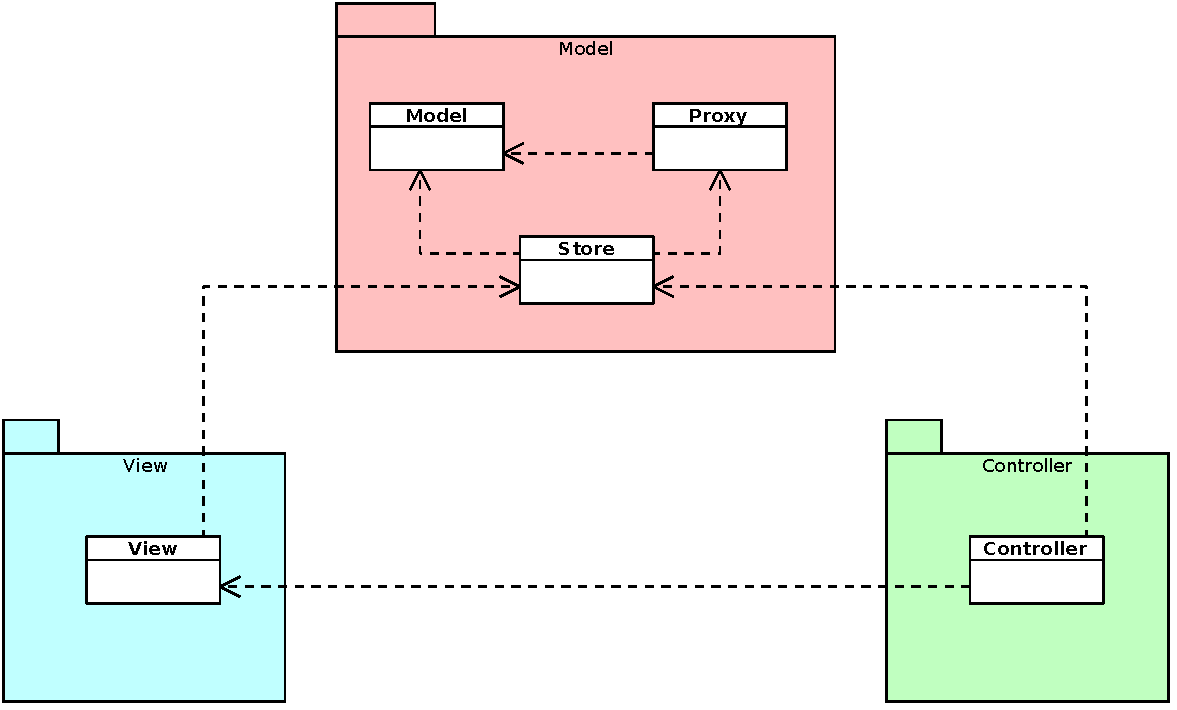
\includegraphics[scale=0.6]{gfx/class/Sencha_Touch_2.pdf}
\caption{Architettura generale Sencha Touch 2}
\label{fig:architettura Sencha}
\end{figure}
Il diagramma in figura \ref{fig:architettura Sencha} rappresenta l'architettura generale che ogni applicazione deve avere, ciò è riflesso anche nella struttura di cartelle e nei nomi dei file; essa si basa sul pattern architetturale \ac{MVC} composto da \emph{model}, \emph{view} e \emph{controller} al quale i progettisti \emph{Sencha} hanno apportato alcune modifiche: è stato aggiunto un componente chiamato \emph{store} che si occupa di separare il prototipo dei dati dai metodi di accesso agli stessi; tale pattern è quindi composto da 4 package che svolgono funzioni diverse:
\begin{description}
\item[model:] rappresenta il modello dei dati su cui si basa l'applicazione; ogni oggetto \emph{model} viene gestito da uno \emph{store} che si occupa di leggere e scrivere i dati mediante un \emph{proxy};
\item[store:] rappresenta una collezione di istanze di modelli e viene utilizzato per gestire caricamento, modifica e salvataggio dei dati dell'applicazione tramite un \emph{proxy};
\item[view:] rappresenta tutti gli oggetti che servono a visualizzare le informazioni all'utente e si riflette dunque sull'interfaccia grafica;
\item[controller:] rappresenta il gestore della logica dell'applicazione; esegue il collegamento tra l'azione che l'utente desidera svolgere e i dati effettivi sul quale l'azione deve essere eseguita.
\end{description}

\section{MyNotes}
\begin{figure}[htbp]
\centering
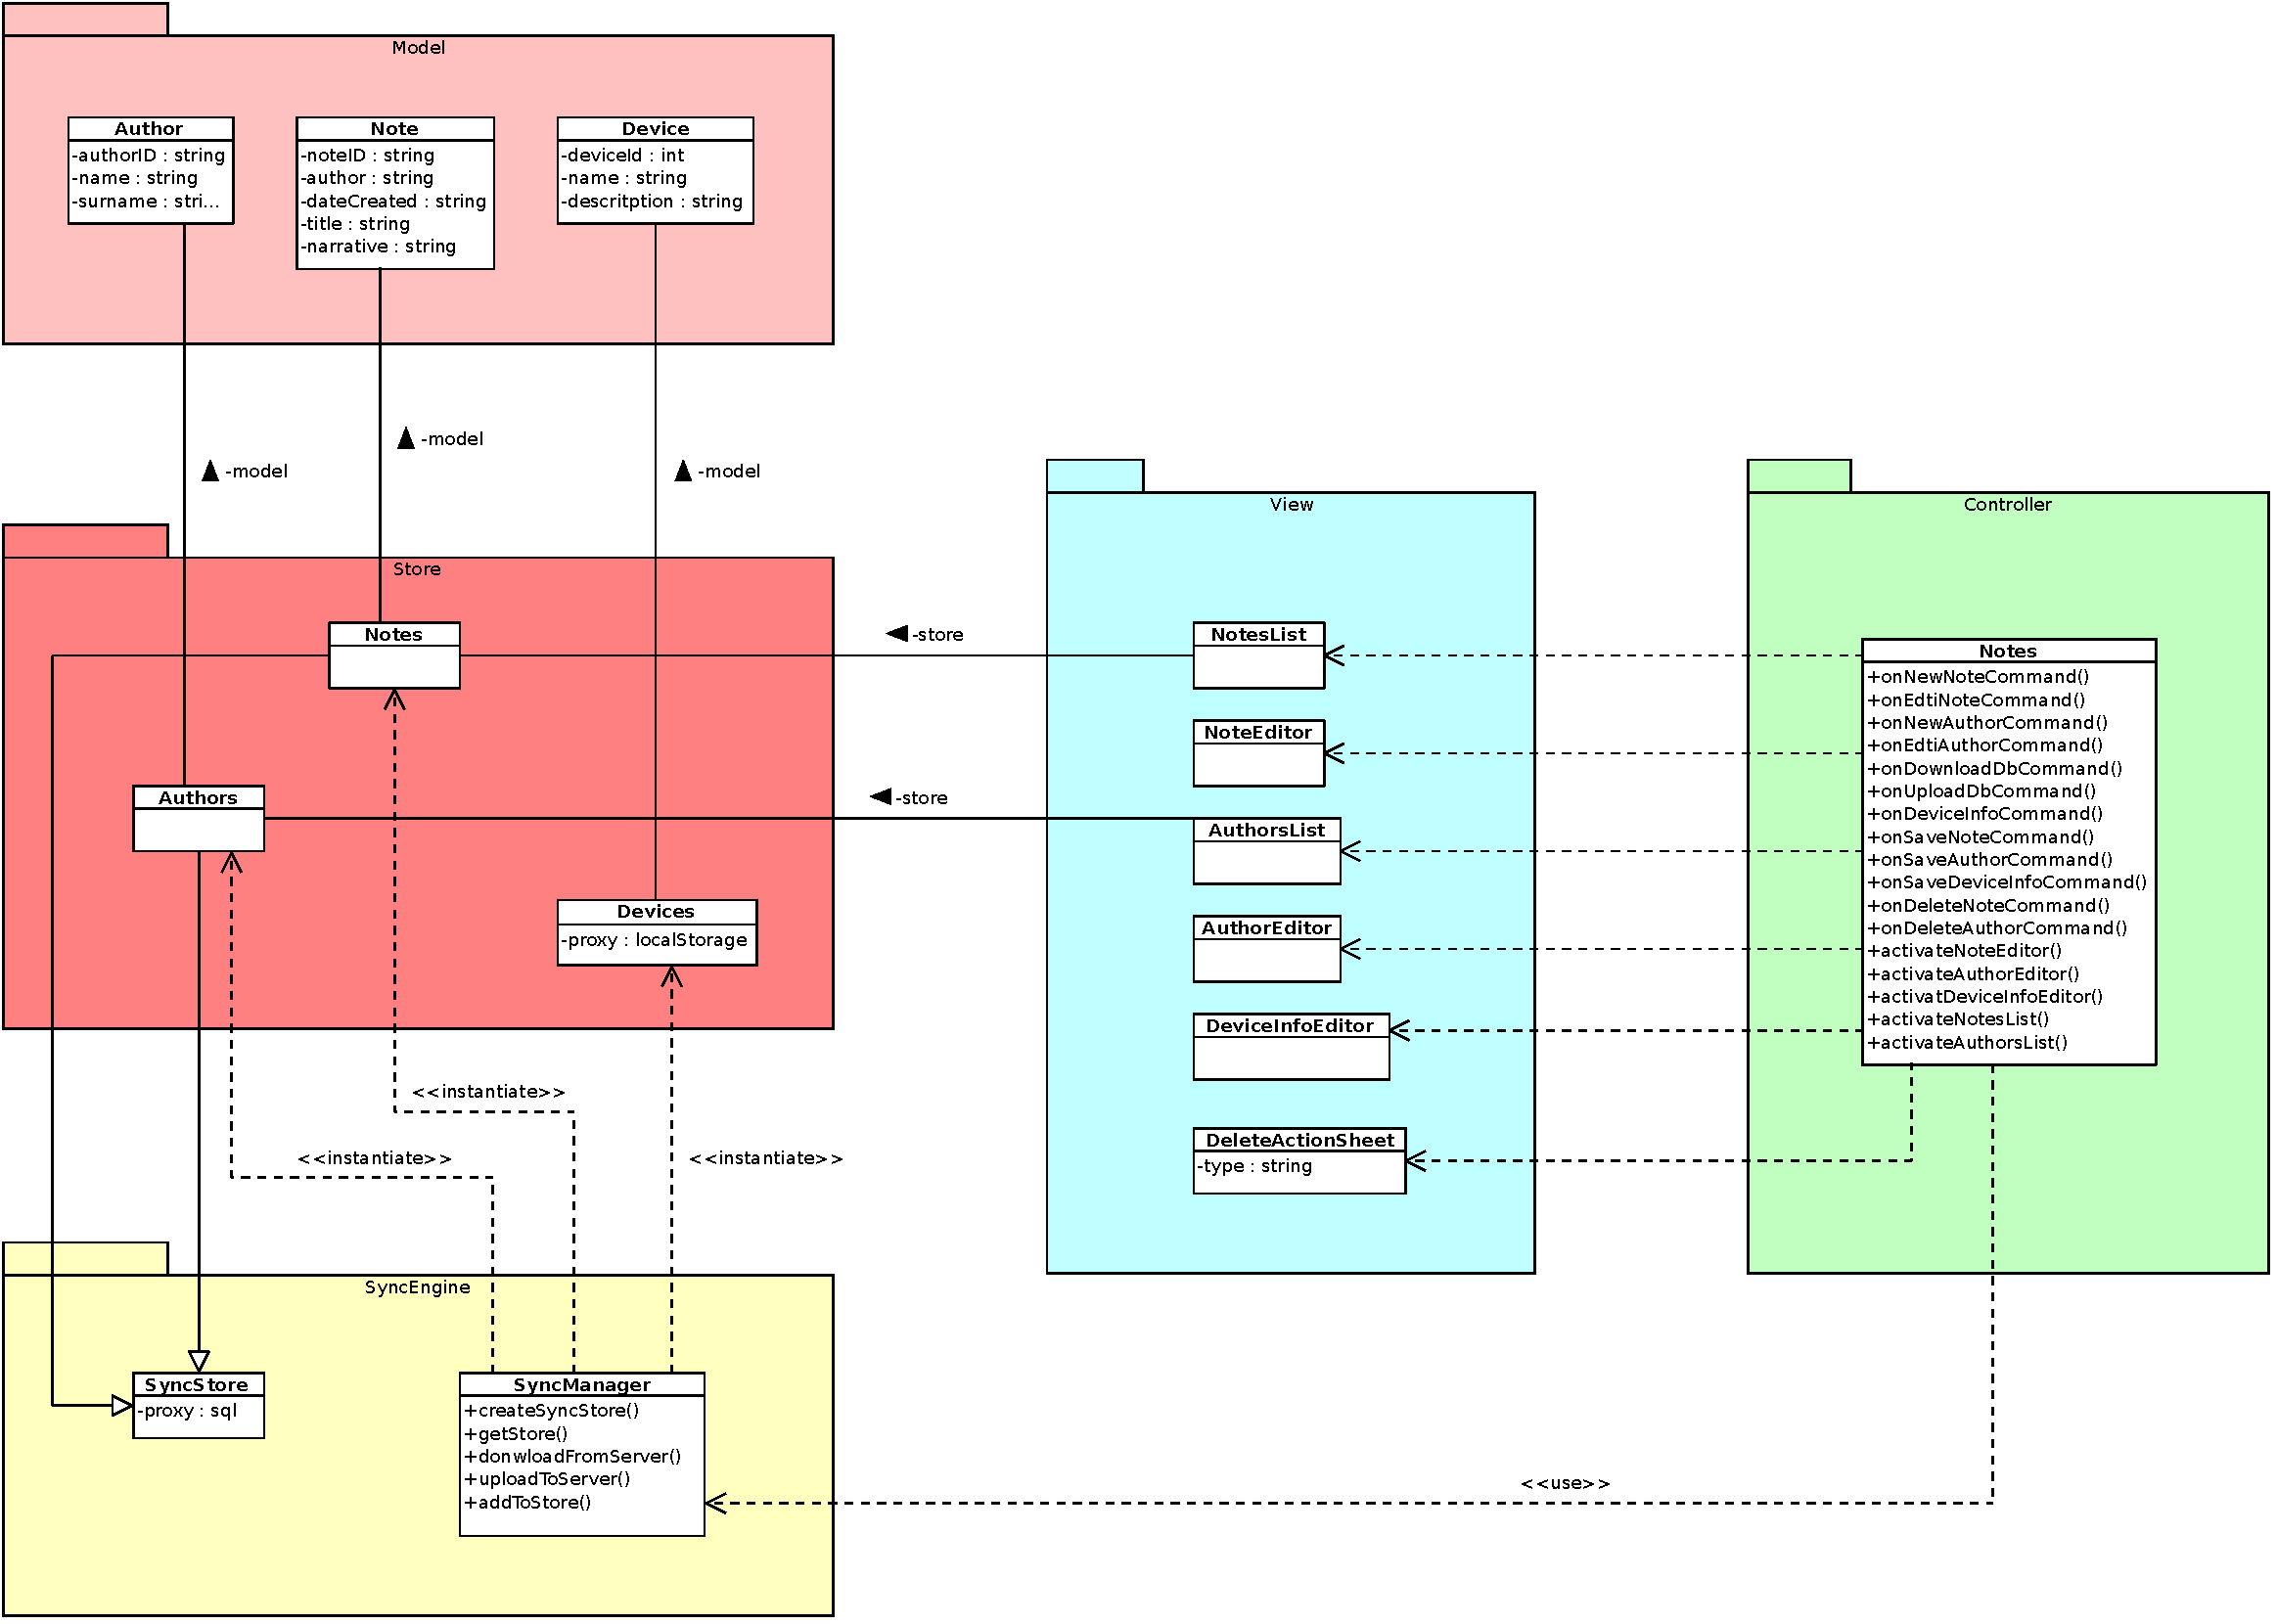
\includegraphics[scale=0.5,angle=90]{gfx/class/MyNotes.pdf}
\caption{Architettura generale -- MyNotes}
\label{fig:architettura MyNotes}
\end{figure}
L'architettura generale dell'applicazione \emph{MyNotes} è rappresentata in figura \ref{fig:architettura MyNotes} ed evidenzia le dipendenze esistenti tra i package individuati.

Dal diagramma si evince come non ci siano gerarchie tra i componenti, ma ogni prototipo rappresenta un'entità particolare con compiti specifici che vengono gestiti dal controller; ognuno di questi oggetti, esclusi il controller e il \emph{SyncManager}, interagisce con al più un altro oggetto, il che rende semplice l'organizzazione dei componenti.

\subsection{Model - Store}
\begin{figure}[htb]
\centering
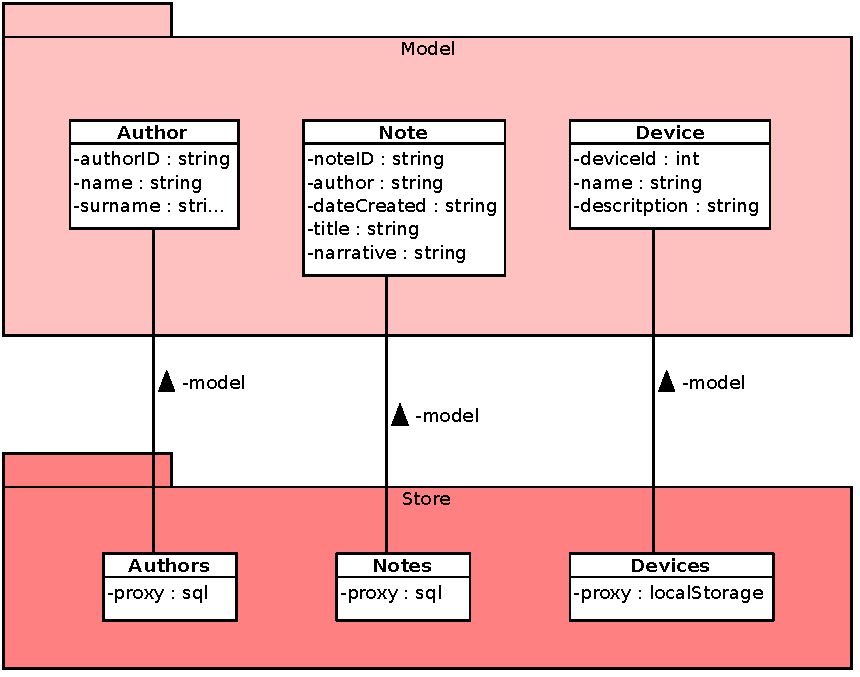
\includegraphics[scale=0.6]{gfx/class/MyNotes_Model_Store.pdf}
\caption{Architettura generale -- MyNotes Model - Store}
\label{fig:architettura MyNotes Model-Store}
\end{figure}
Per soddisfare i requisiti e quindi la necessità di gestire note, autori e device si sono progettati tre modelli omonimi con i relativi store.
I modelli in questione sono molto semplici e contengono pochi campi in quanto non rappresentano un'entità reale ma solo dimostrativo.

Per autori e note si è scelto di utilizzare il proxy di tipo \emph{sql} il quale usa \emph{SQLite} per il salvataggio dei dati; la scelta è stata obbligata in quanto il \emph{SyncManager} utilizza tale tipo di proxy.
Per quanto riguarda le informazioni del dispositivo invece è sufficiente un proxy di tipo \emph{localStorage} in quanto non necessita di essere sincronizzato e può essere gestito localmente.

\subsection{View}
\begin{figure}[htb]
\centering
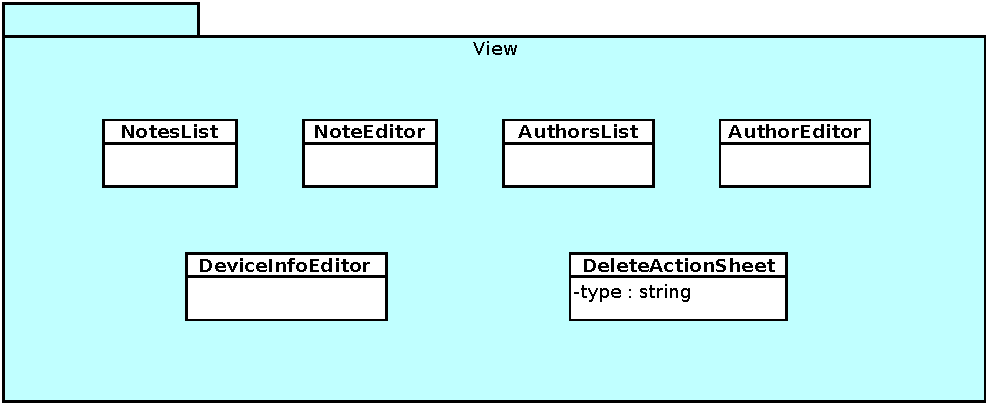
\includegraphics[scale=0.6]{gfx/class/MyNotes_View.pdf}
\caption{Architettura generale -- MyNotes View}
\label{fig:architettura MyNotes View}
\end{figure}
Le viste progettate sono dei componenti che vengono utilizzati per visualizzare la lista delle note, \emph{NotesList}, e degli autori, \emph{AuthorsList} e per gestire creazione e modifica di note, \emph{NoteEditor}, autori, \emph{AuthorEditor}, e delle informazioni del dispositivo, \emph{DeviceInfoEditor}.

È presente un ulteriore vista, \emph{DeleteActionSheet}, che ha il compito di richiedere la conferma dell'eliminazione di una nota o di un autore all'utente; tale componente è in grado di distinguere il tipo del dato che l'utente desidera eliminare tramite il parametro \emph{type}.

\subsection{Controller}
\begin{figure}[htb]
\centering
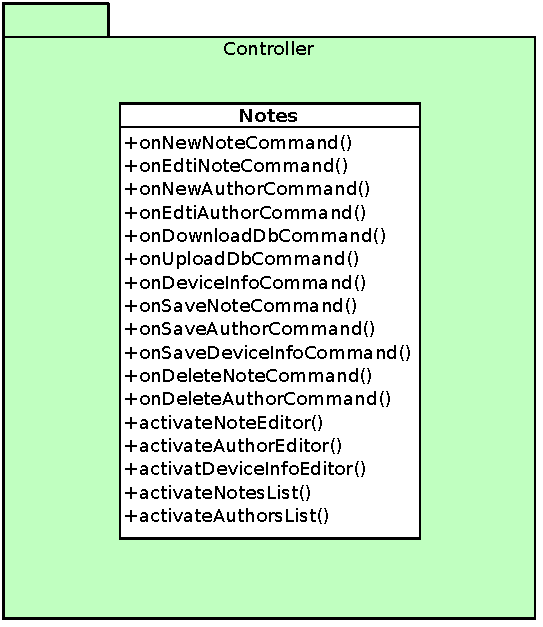
\includegraphics[scale=0.6]{gfx/class/MyNotes_Controller.pdf}
\caption{Architettura generale -- MyNotes Controller}
\label{fig:architettura MyNotes Controller}
\end{figure}
Il \emph{Controller} è il componente più significativo dell'applicazione e viene utilizzato per catturare tutti gli eventi generati dalle viste all'interazione dell'utente con un componente grafico.

Esso infatti dispone dei riferimenti a tutte le viste esistenti ed utilizza dei metodi di controllo per svolgere le diverse operazioni di caricamento, elaborazione e salvataggio dei dati.

Inoltre svolge il suo compito in stretta relazione con il \emph{SyncManager} per quanto riguarda la gestione degli store, infatti, ogni operazione su di essi è mediata da questo componente che svolge la funzione di intermediario con il \emph{SyncEngine} rendendo trasparente allo sviluppatore la gestione dei dati.

\subsection{SyncEngine}
\begin{figure}[htb]
\centering
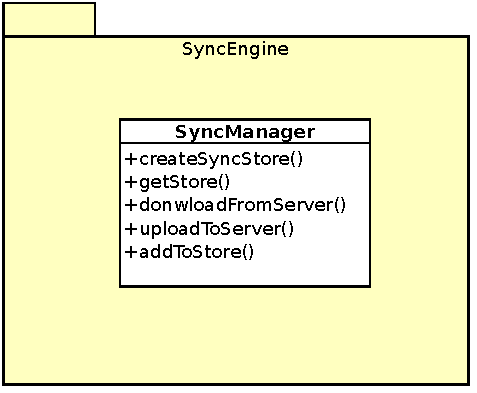
\includegraphics[scale=0.6]{gfx/class/SyncEngine.pdf}
\caption{Architettura generale -- MyNotes SyncEngine}
\label{fig:architettura MyNotes SyncEngine}
\end{figure}
Il \emph{SyncEngine} è un componente che permette di creare dinamicamente degli store legati a modelli statici presenti nell'applicazione, con lo scopo di sincronizzarli con un server remoto adeguatamente predisposto.

Per gestire ed utilizzare correttamente questo componente è stata predisposta un'interfaccia denominata \emph{SyncManager} dalla quale è possibile creare gli store necessari e utilizzarli in modo ottimale all'interno dell'applicazione: sarà quindi possibile utilizzarli per leggere e salvare i dati e per effettuare la sincronizzazione con quelli presenti nel server.

\section{SensorDevice}
\begin{figure}[htb]
\centering
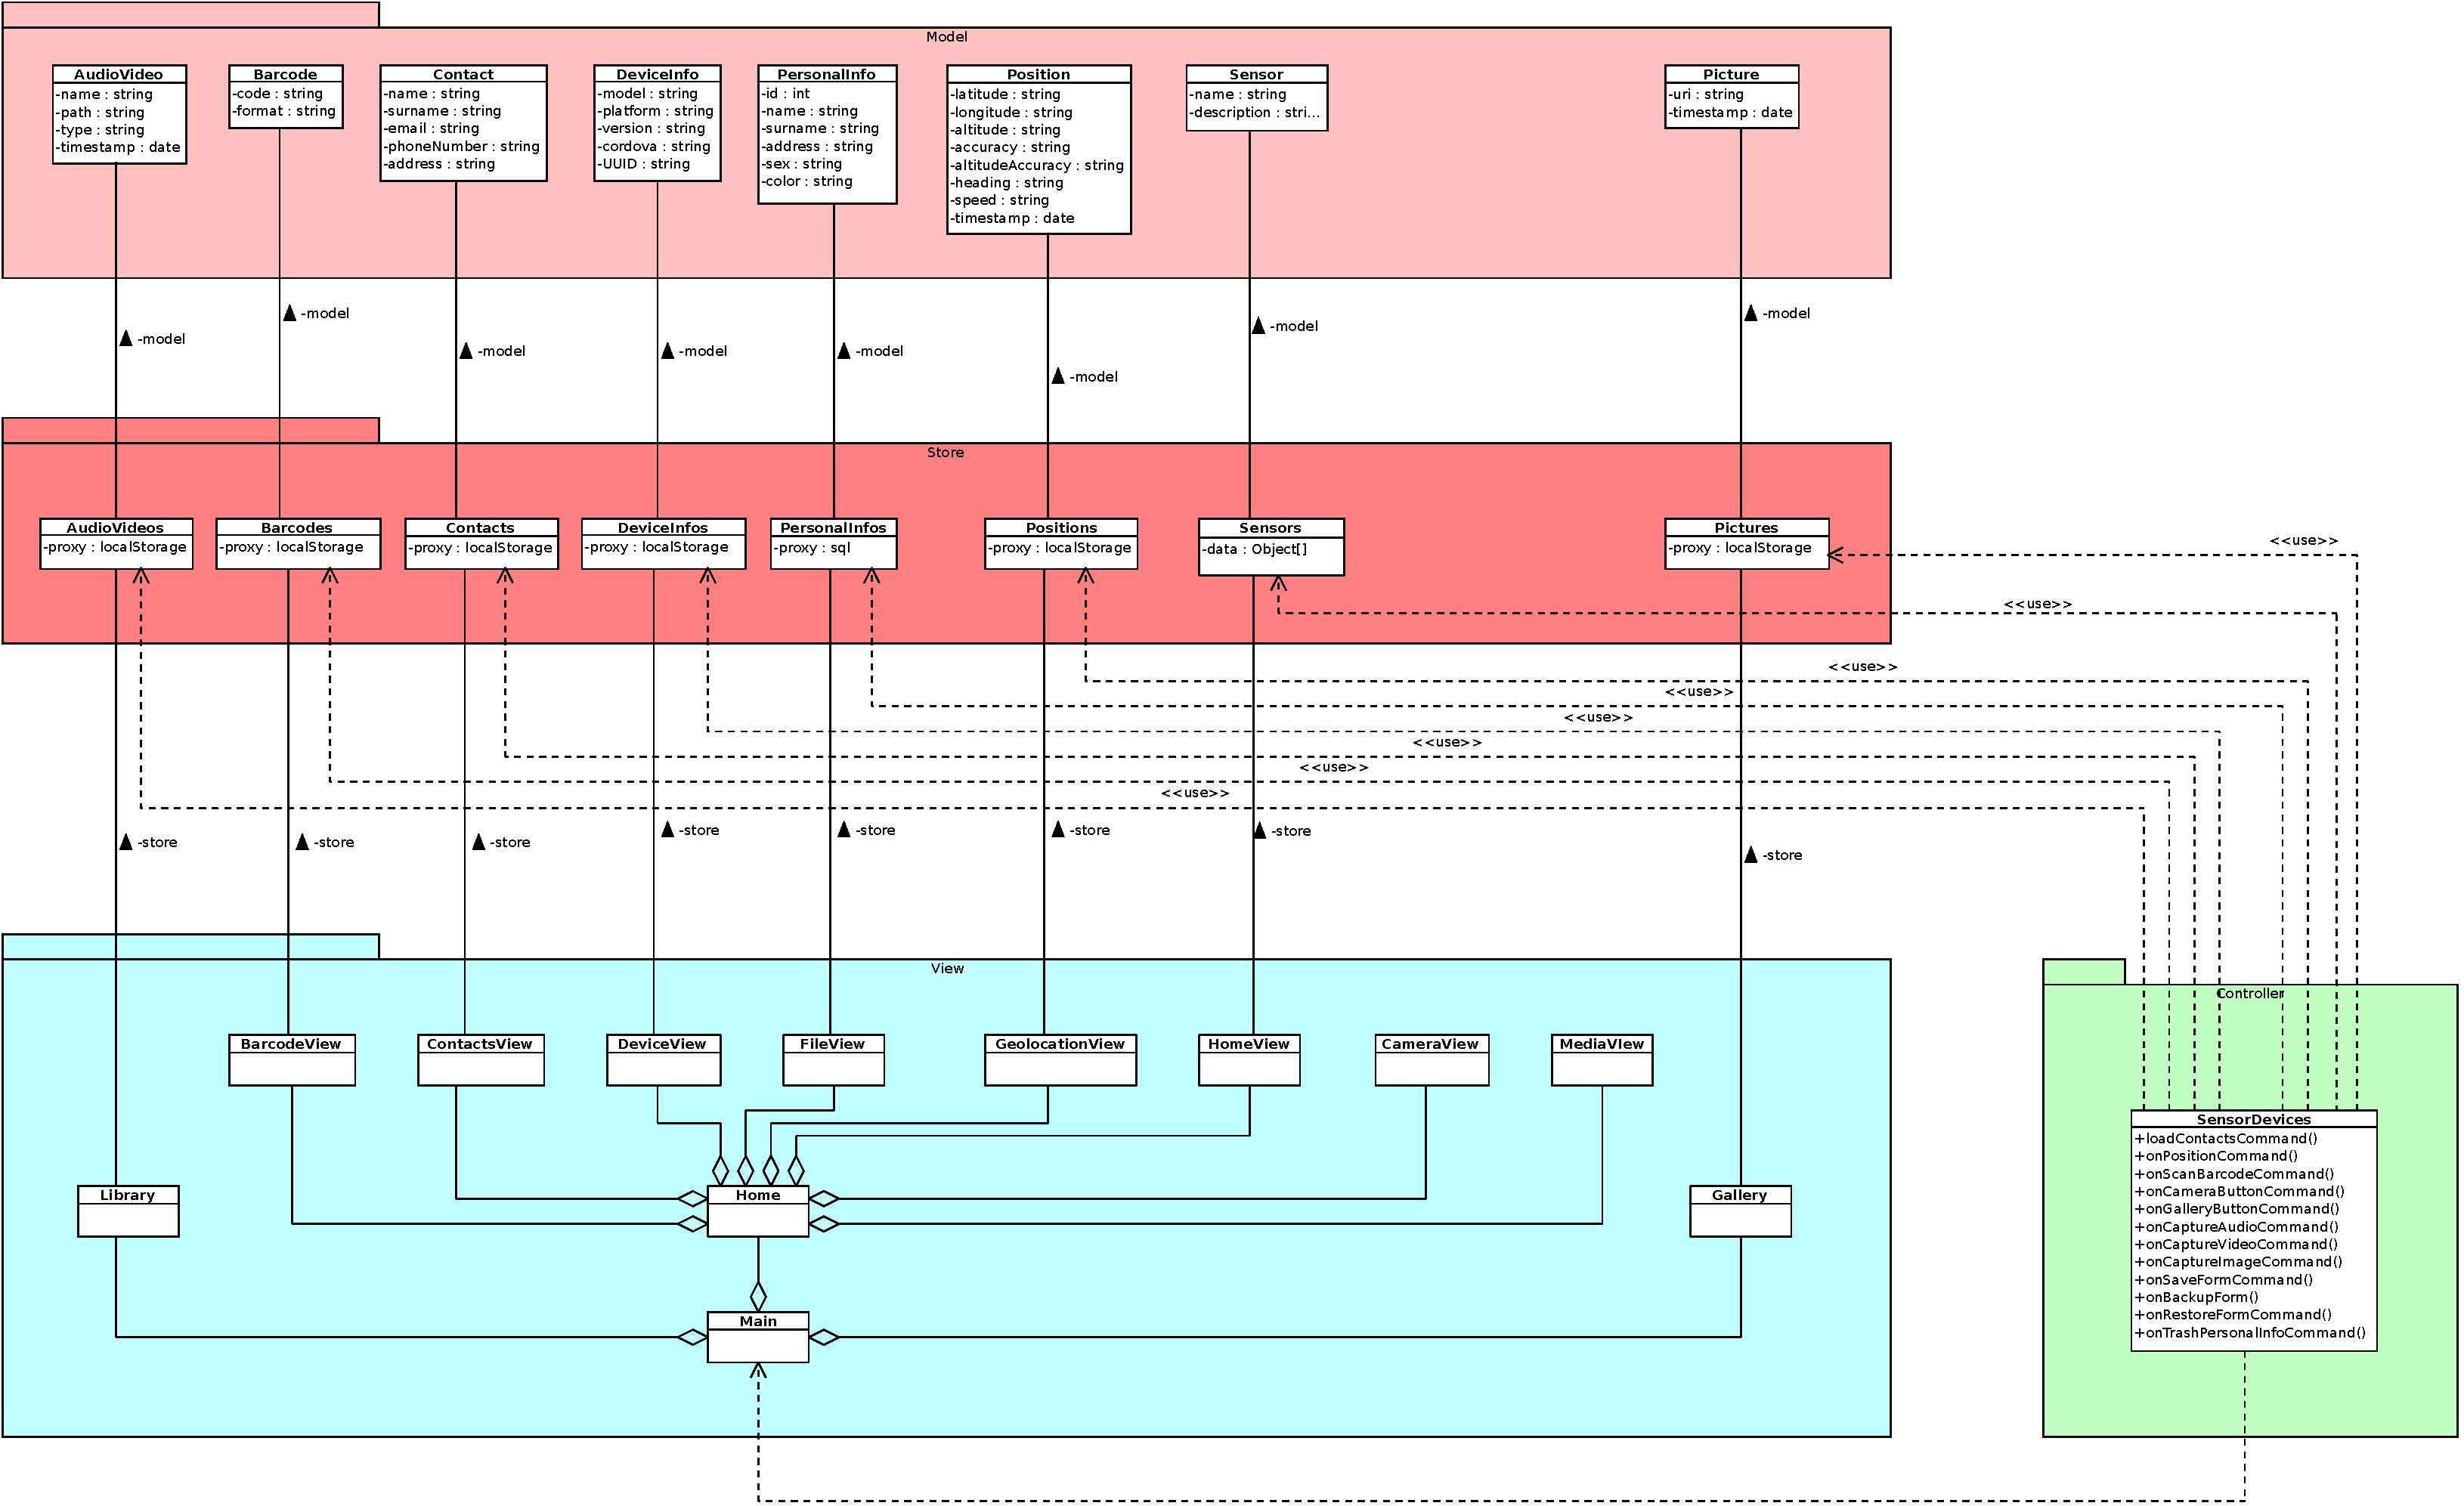
\includegraphics[scale=0.4,angle=90]{gfx/class/SensorDevice.pdf}
\caption{Architettura generale -- SensorDevice}
\label{fig:architettura SensorDevice}
\end{figure}
In figura \ref{fig:architettura SensorDevice} è rappresentata l'architettura ad alto livello dell'applicazione \emph{SensorDevice}: utilizza il pattern architetturale \ac{MVC} che contraddistingue tutte le applicazioni sviluppate con \emph{Sencha Touch}.

Come per \emph{MyNotes} non esistono gerarchie di tipi e il rapporto tra modelli e store è sempre di 1 a 1; si può notare, inoltre, come le viste siano particolarmente articolate a causa della necessità di visualizzare una notevole quantità di dati che vengono raccolti dal sistema.

\subsection{Model - Store}
\begin{figure}[htb]
\centering
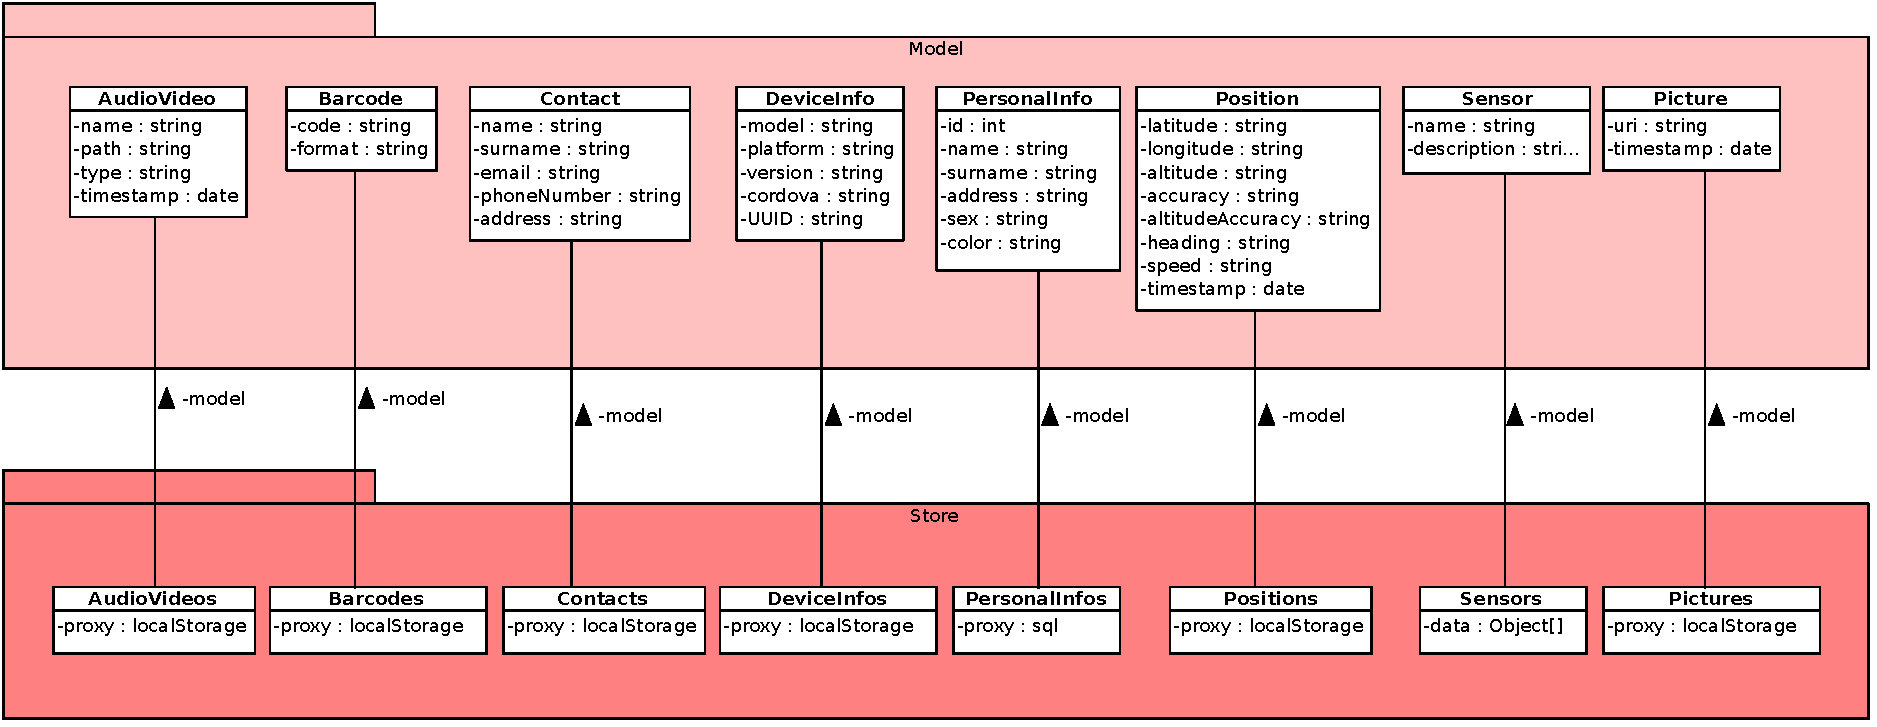
\includegraphics[scale=0.4]{gfx/class/SensorDevice_Model_Store.pdf}
\caption{Architettura generale -- SensorDevice Model - Store}
\label{fig:architettura SensorDevice Model-Store}
\end{figure}
Per soddisfare le richieste dell'azienda sono stati progettati sette modelli diversi, ognuno rappresentante della funzionalità da sviluppare, più il modello \emph{Sensor} che viene utilizzato solamente per creare una lista delle funzionalità che l'utente può decidere di utilizzare nella pagina principale dell'applicazione.

Ogni modello ha associato uno store con proxy di tipo \emph{localStorage}, tranne \emph{PersonalInfos} che ne possiede uno di tipo \emph{sql}, in quanto, tramite il relativo modello, si intende testare il backup e il ripristino dei dati sulla memoria di massa del dispositivo che verrà effettuato tramite un file di testo.

\subsection{View}
\begin{figure}[htb]
\centering
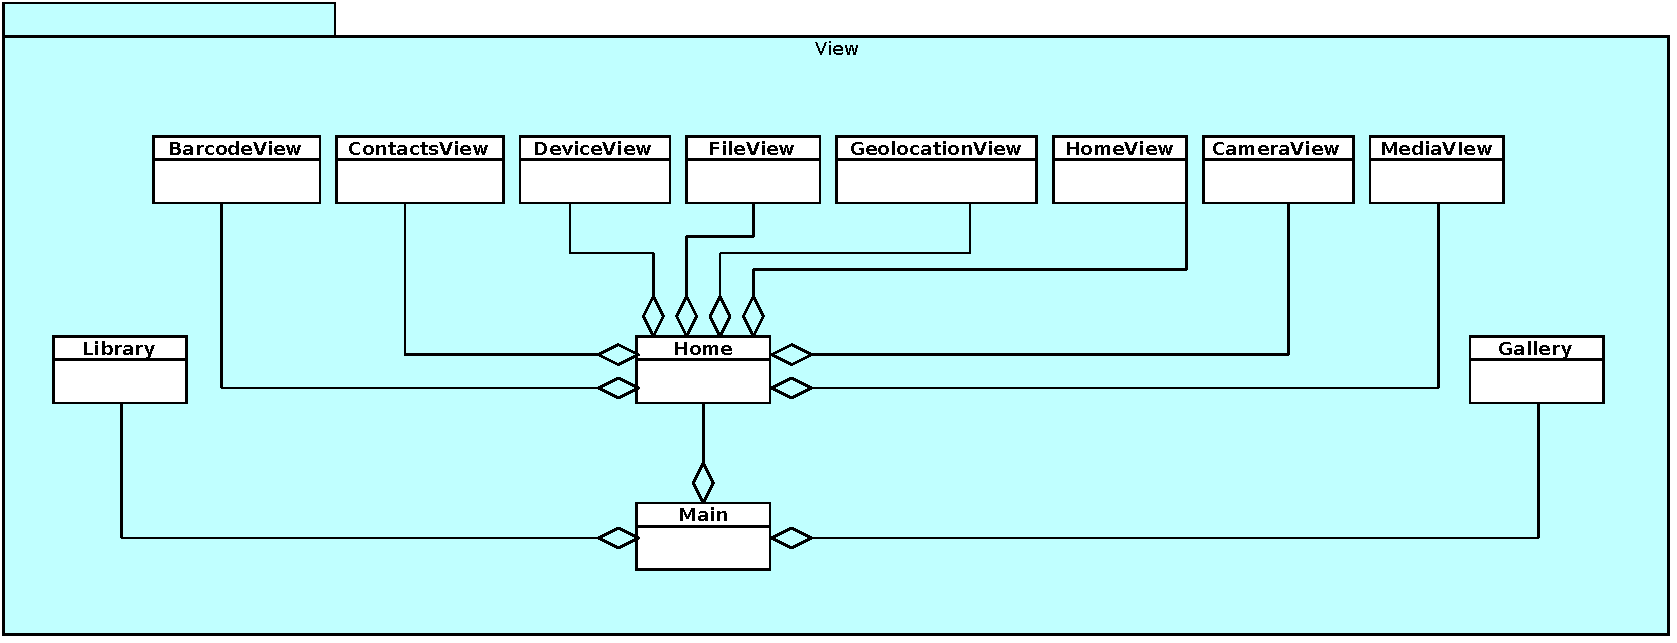
\includegraphics[scale=0.45]{gfx/class/SensorDevice_View.pdf}
\caption{Architettura generale -- SensorDevice View}
\label{fig:architettura SensorDevice View}
\end{figure}
Come si evince dalla figura \ref{fig:architettura SensorDevice View} si è scelto di creare una vista per ogni funzionalità da sviluppare, in modo da rendere più agevole all'utente la consultazione dei dati catturati, e di raggruppare queste in una pagina principale, chiamata \emph{Home}, dalla quale è possibile navigare tutte le viste.

Inoltre sono state progettate due pagine dedicate alla visualizzazione di immagini, \emph{Gallery}, e di video e audio, \emph{Library}.
Si è deciso di dividere le due categorie di \emph{media} in quanto necessitano di una diversa gestione per essere visualizzati o riprodotti.

\subsection{Controller}
\begin{figure}[htb]
\centering
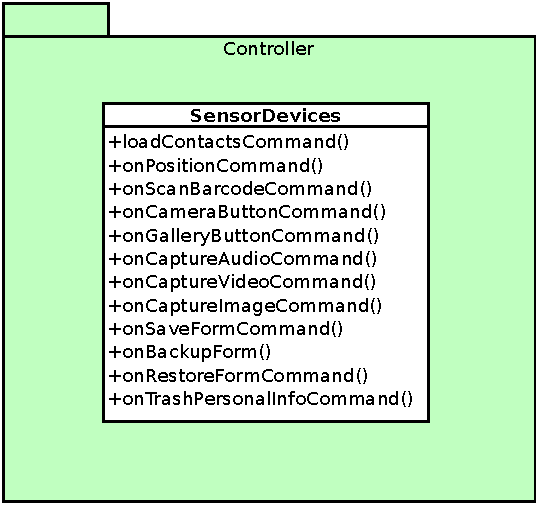
\includegraphics[scale=0.6]{gfx/class/SensorDevice_Controller.pdf}
\caption{Architettura generale -- SensorDevice Controller}
\label{fig:architettura SensorDevice Controller}
\end{figure}
Come per \emph{MyNotes}, il controller possiede riferimenti alle viste dell'applicazione e cattura gli eventi da loro generati, i quali vengono gestiti mediante i metodi predisposti.

In questa applicazione il controller gestisce direttamente creazione e modifica degli store in quanto non è presente nessun componente intermedio come accade per \emph{MyNotes}.